% begin module improper-integral-geometry

\begin{frame}
\frametitle{Type I: Infinite Intervals}
\begin{itemize}
\item  Consider the region $A$ that lies under $y = 1/x^2$, above the $x$-axis, and to the right of $x = 1$.
\item<2->  To find its area, approximate with $A(t)$, the area of the region under $1/x^2$, above the $x$-axis, right of $x = 1$, and left of $x = t$.
\end{itemize}
\begin{columns}[c]
\column{.5\textwidth}
\[
\uncover<2->{%
A(t) = \int_1^t \frac{\diff x}{x^2} = %
}%
\uncover<3->{%
\left[ -\frac{1}{x}\right]_1^t = %
}%
\uncover<4->{%
1 - \frac{1}{t}
}%
\]
\column{.5\textwidth}

\psset{xunit=1cm, yunit=1cm}
\begin{pspicture}(-0.5, -0.5)(5.6,2.1)
\psframe*[linecolor=white](-0.5,-0.5)(5.6,2.1)
\tiny
\uncover<1,14->{
\psline[linewidth=0.5pt](1,0)(1,1)
\pscustom*[linecolor=\fcColorAreaUnderGraph]{
\psplot[linecolor=\fcColorGraph, plotpoints=1000]{1}{5.5}{1 x 2 exp div }
\psline(5.5,0.033057851)(5.5, 0)(1,0)
}
}

\uncover<2-9>{
\pscustom*[linecolor=\fcColorAreaUnderGraph]{
\psplot[linecolor=\fcColorGraph, plotpoints=1000]{1}{3}{1 x 2 exp div }
\psline(3,  0.111111)(3, 0)(1,0)
}
\psline[linewidth=0.5pt](3,  0.111111)(3, 0)
\fcXTickWithLabel{3}{$t$}
}

\uncover<handout:0|10>{
\pscustom*[linecolor=\fcColorAreaUnderGraph]{
\psplot[linecolor=\fcColorGraph, plotpoints=1000]{1}{2}{1 x 2 exp div }
\psline(2,  0.25)(2, 0)(1,0)
}
\psline(2,0)(2, 0.25)
\fcXTickWithLabel{2}{$2$}
}

\uncover<handout:0|11>{
\pscustom*[linecolor=\fcColorAreaUnderGraph]{
\psplot[linecolor=\fcColorGraph, plotpoints=1000]{1}{3}{1 x 2 exp div }
\psline(3,  0)(1,0)
}
\psline(3,0)(3, 0.111111)
\fcXTickWithLabel{3}{$3$}
}
\uncover<handout:0|12>{
\pscustom*[linecolor=\fcColorAreaUnderGraph]{
\psplot[linecolor=\fcColorGraph, plotpoints=1000]{1}{4}{1 x 2 exp div }
\psline(4,  0)(1,0)
}
\psline(4,0)(4, 0.0625)
\fcXTickWithLabel{4}{$4$}
}
\uncover<handout:0|13>{
\pscustom*[linecolor=\fcColorAreaUnderGraph]{
\psplot[linecolor=\fcColorGraph, plotpoints=1000]{1}{5}{1 x 2 exp div }
\psline(5,  0)(1,0)
}
\psline(5,0)(5, 0.04)
\fcXTickWithLabel{5}{$5$}
}


\psaxes[ticks=none, labels=none]{<->}(0,0)(-0.5,-0.5)(5.5,2)
\fcLabels{5.5}{2}
%Function formula: (1)/((x)^{2})
\rput[b](5,0.3){$y=\frac{1}{x^2}$}
\psplot[linecolor=\fcColorGraph, plotpoints=1000]{0.75}{5.5}{1 x 2 exp div }

%\uncover<1,14->{\rput(1.7, 1.2){$A$}}

\rput[l](1.7, 1.2){$\displaystyle\uncover<1,2-9,14>{ A} \uncover<2-9>{(t)} \uncover<4-9>{=1-\frac{1}t}$}
\uncover<handout:0|10>{\rput[l](1.7, 1.2){$\displaystyle A(2)=\frac{1}2$}}
\uncover<handout:0|11>{\rput[l](1.7, 1.2){$\displaystyle A(3)=\frac{2}3$}}
\uncover<handout:0|12>{\rput[l](1.7, 1.2){$\displaystyle A(4)=\frac{3}4$}}
\uncover<handout:0|13>{\rput[l](1.7, 1.2){$\displaystyle A(5)=\frac{4}5$}}

%\uncover<2-9>
{\psline[linewidth=2pt]{->}(1.6, 0.9 )(1.2, 0.3)}
\fcXTickWithLabel{1}{$1$}
\psline[linewidth=0.5pt](1,  0)(1, 1)

\end{pspicture}
%\ \only<-1>{%
%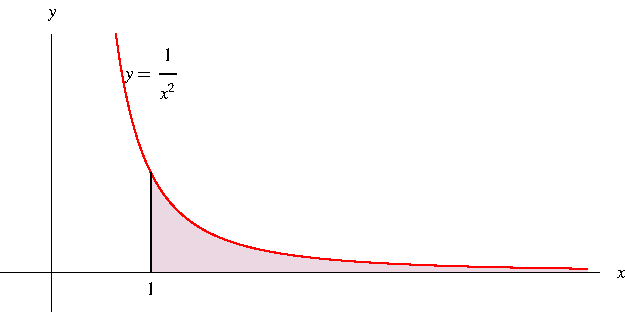
\includegraphics[height=3cm]{improper-integrals/pictures/08-08-xsquaredy.pdf}%
%}%
%\only<handout:0| 2-3>{%
%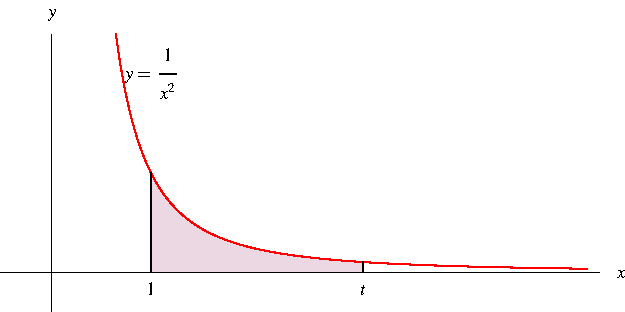
\includegraphics[height=3cm]{improper-integrals/pictures/08-08-xsquaredz.pdf}%
%}%
%\only<handout:0| 4-8>{%
%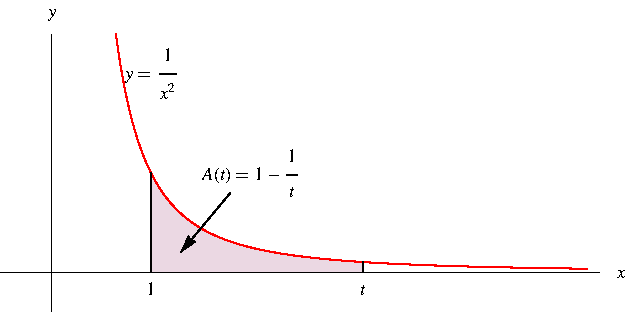
\includegraphics[height=3cm]{improper-integrals/pictures/08-08-xsquareda.pdf}%
%}%
%\only<handout:0| 9>{%
%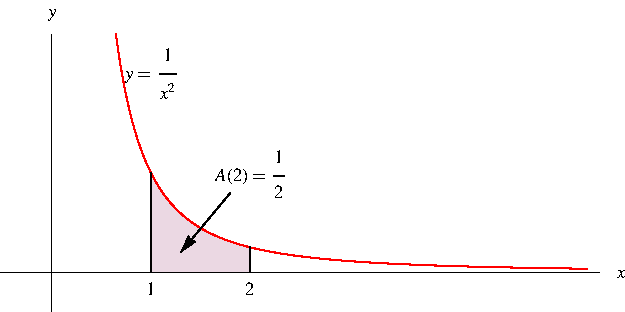
\includegraphics[height=3cm]{improper-integrals/pictures/08-08-xsquaredb.pdf}%
%}%
%\only<handout:0| 10>{%
%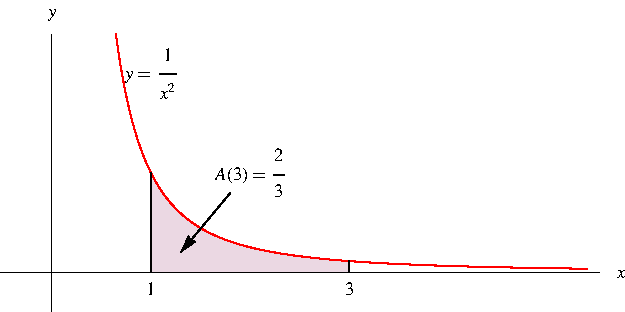
\includegraphics[height=3cm]{improper-integrals/pictures/08-08-xsquaredc.pdf}%
%}%
%\only<handout:0| 11>{%
%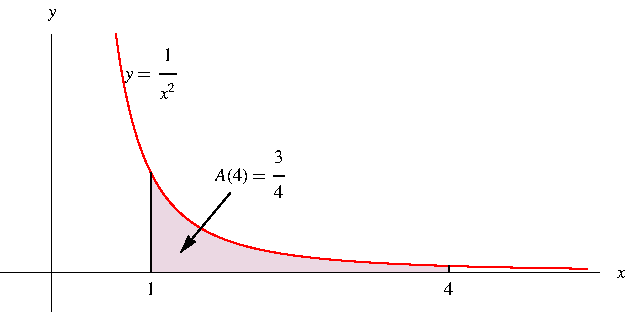
\includegraphics[height=3cm]{improper-integrals/pictures/08-08-xsquaredd.pdf}%
%}%
%\only<handout:0| 12>{%
%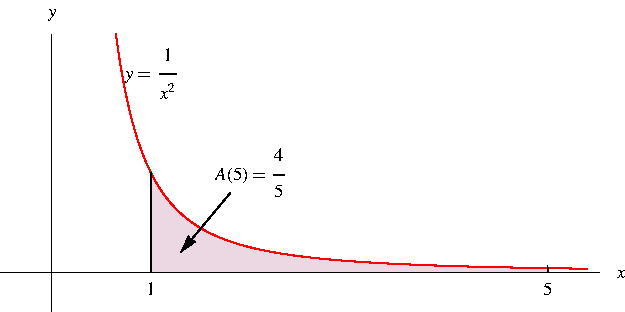
\includegraphics[height=3cm]{improper-integrals/pictures/08-08-xsquarede.pdf}%
%}%
%\only<handout:0| 13->{%
%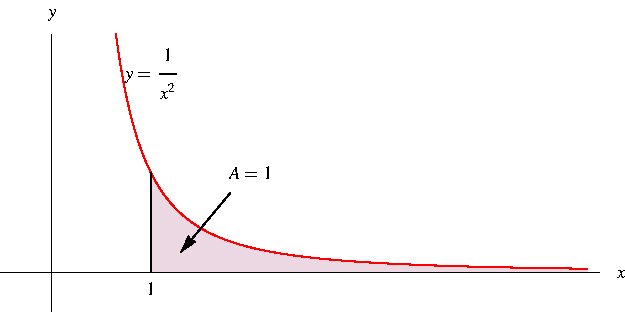
\includegraphics[height=3cm]{improper-integrals/pictures/08-08-xsquaredf.pdf}%
%}%
\end{columns}
\begin{itemize}
\item<5->  Notice $A(t) < 1$ no matter how large $t$ is.
\item<6->  Also notice $\lim\limits_{t\rightarrow \infty}A(t) = \alert<handout:0| 7-8>{\lim\limits_{t\rightarrow \infty}\left( 1 - \frac{1}{t}\right) = \fcAnswer{8}{1}}$\uncover<8->{.}
\item<14->  We say that the area $A$ is equal to $1$ and write $\int_1^\infty \frac{1}{x^2}\diff x = \lim_{t\rightarrow \infty}\int_1^t \frac{1}{x^2}\diff x = 1$.
\end{itemize}
\end{frame}
% end module improper-integral-geometry
